\chapter{Experimental Analysis}

The following is a description of the environment that has been set up for the fault injection tests, by means of chosen benchmark applications and the hardware design preparation behind the related choices. The second part of this chapter illustrates in detail the obtained experimental results, highlighting some interesting considerations.

\section{Fault Injection Environment}

Before proceeding with the fault injection campain, aimed to demonstrate the effectiveness of the developed fault tolerance design, the Fault Injection Tool requires some extra hardware for a good understing of the obtained results.

\subsubsection{Watchdog Configuration}
The watchdog IP, during the design stage, is configured through its customization wizard with a default timeout value of 2 seconds (two times the clock frequency) and it is started by default. This choice has been taken because under normal operational conditions, the MicroBlaze is capable of starting the watchdog and set a correct timeout value.\bigskip
 
Instead, with the choosen fault injection method, the MicroBlaze directly starts with a bit-flip in his configuration, hence it may be not able to start correctly the watchdog or to set a valid timeout value. Therefore, the campaign results would not be valid.\bigskip

\subsubsection{Hardware to count the number of timeouts}
In order to understand if the watchdog is capable of covering a good number of faults by expiring, the design has been equipped with a UP counter. The counter is reseted everytime the FGPA is programmed with a new full bitstream. The counter is incremented everytime the watchdog expires by connecting the CLK port to the timeout signal, and its value is obtained via a AXI GPIO peripheral that is connected to the AXI Interconnect. \bigskip

\begin{figure}[H]
\centering
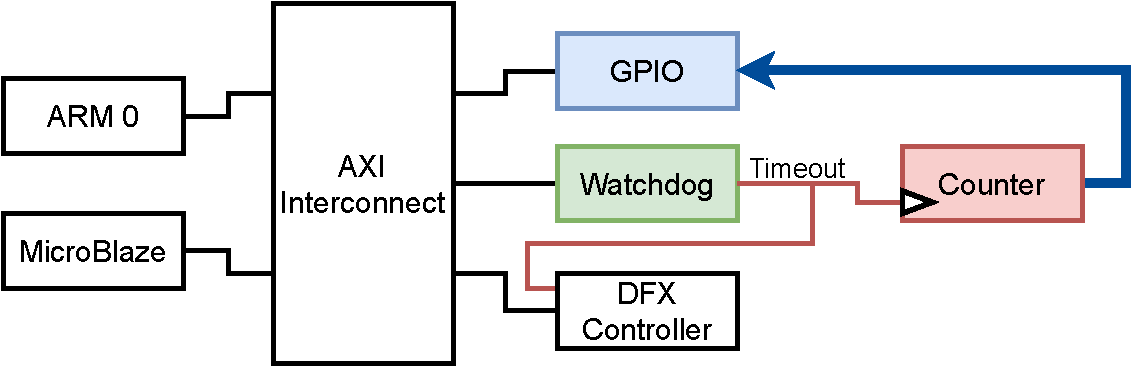
\includegraphics[width=0.95\linewidth]{images/chapter5/upc.pdf}
\caption{Hardware schematic to count the number of times the watchdog time outs.}
\end{figure}

Both the MicroBlaze and the PS can access it. Because the MicroBlaze is under test and may not be able to access correctly the GPIO peripheral, the value is read from one of the ARM cores in the PS side.\bigskip

% UP-counter added to read the number of times the reconf is triggered (clk connected to trigger). Count accessed via a GPIO memory mapped from the ARM core.

\subsubsection{Benchmark Firmware}

As explained in previous sections, a good benchmark software is required for a good fault injection campaign for two reasons:
\begin{itemize}
    \item A good benchmark is able to stress various aspects of the MicroBlaze's hardware (ALU, Decode Unit, Controller Unit, etc.) and reveal a hidden fault.
    \item A good benchmark is able to self-test itself (checking the correctness of the produced results).
\end{itemize}

The following is an extract of the firmware running on the MicroBlaze, that computes the Fibonacci series up to a certain point and checks the results via a simple checksum check:

\begin{lstlisting}[style=C]
int main() {
  int i;
  uint64_t op1 = 0, op2 = 0, res = 0, checksum = 0;
  GBcnCtrl hBcn;

  i = XPAR_BEACON_WATCHDOG_0_S00_AXI_BASEADDR;
  GBcnCtrl_Initialize(&hBcn, i);

  print("started? ", GBcnCtrl_IsStarted(&hBcn) ? 1 : -1);
  i = hBcn.modules->module0.DATAREG;
  print("timeout: ", i ? i : -1);
  GBcnCtrl_SetTimeoutValue(&hBcn, XPAR_CPU_CORE_CLOCK_FREQ_HZ<<1);
  GBcnCtrl_Start(&hBcn);
  print("started? ", GBcnCtrl_IsStarted(&hBcn) ? 1 : -1);
  i = hBcn.modules->module0.DATAREG;
  print("timeout: ", i ? i : -1);

  op1 = op2 = 1;
  print("Fibonacci current value ", op1);
  print("Fibonacci current value ", op2);

  while(1) {
    checksum ^= (res = op1 + op2);
    if(res > 0xfffff) {
  	  res = 1;
  	  op2 = 0;
  	  print("\n\rDONE_1 DONE_1 DONE_1\r\n");
  	  break;
    }

    print("Fibonacci current value ", (uint64_t)res);
    op1 = op2;
    op2 = res;
    for (i = 0; i < 1e5; i++); // a bit of delay
    GBcnCtrl_Toggle(&hBcn);
  }

  printt("CHECKSUM: ", checksum);
  if (checksum == 1673873) {
    print("DONE_2 DONE_2 DONE_2\r\n");
    for (i = 0; i < 5e6; i++); // delay
    GBcnCtrl_Toggle(&hBcn); // all fine!
  } else {
    print("WRONG CHECKSUM!\r\n");
    while(1); // stops toggling because wrong checksum
  }
}
\end{lstlisting}

\subsubsection{How the fault injection tool access the number of expired times}

The Fault Injection Tool has been enhanced to support the retrieval of the number of times the watchdog expires at each run. It does it via a XSCT script that appends in a file the retrieved number, as follows:\bigskip

\begin{lstlisting}[style=tcl]
connect -url tcp:127.0.0.1:3121

# selects the ARM #0 core
targets -set -nocase -filter {name =~ "*A9*#0"} 
set outfile1 [open "faulty_bitstreams/uB_results/dfx_cnt.txt" a+]    

# reads the value from the GPIO register
puts $outfile1 [mrd -value 0x41200008 1] 
close $outfile1
\end{lstlisting}

% FI tool generates bitstream -> for each run
% pre\_tcl script to program the bitsteam and the ELF
% post\_tcl to launch the microblaze execution (con comand)
% cnt\_tcl script to obtain the number of reconfigurations triggered (reads from the GPIO mrd 0x41200008)

\section{Experimental Results}

In this section the main obtained results are presented and discussed. During the overall test period, eigth campaigns of fault injection have been performed. Each campaign is made of 100 injections. Some of them are aborted, thus the mean number of completed injections per run is 95, leading to a total of 766 injections. \bigskip

For each fault, there can be three possible outcomes, and each one can have a different reason behind it:
\begin{itemize}
    \item Correct result:
    \begin{enumerate}
        \item The fault has not been triggered so it is naturally masked and the result is automatically correct.
        \item The fault caused a CPU halt (no detected output on the UART). The system corrected the fault and the output is correct. It is identical to the golden one, hence it is marked as correct.
    \end{enumerate}
    \item The output is different from the golden one (SDE):
    \begin{enumerate}
        \item The fault has not been detected by the watchdog, thus it is not fixed.
        \item The MicroBlaze noticed the fault while executing the program and printing messages and it has been fixed. However the output is different from the golden one, even if the final result is correct. Marked as SDE anyway.
        \item The MicroBlaze noticed the fault and tried to fix it, unsuccessfully. The output is different and the result remained incorrect.
    \end{enumerate}
    \item The MicroBlaze is halted:
    \begin{enumerate}
        \item The hangs is detected by the watchdog, but it could not be fixed.
        \item The MicroBlaze does not output nothing on the UART, even if the watchdog is kicked correctly. No output means to hangs but a correct kicking act means that the CPU is working so the reconfiguration is not triggered.
    \end{enumerate}
\end{itemize}

The following one is a summary of the obtained results from the conducted campaigns:

\begin{figure}[H]
\centering
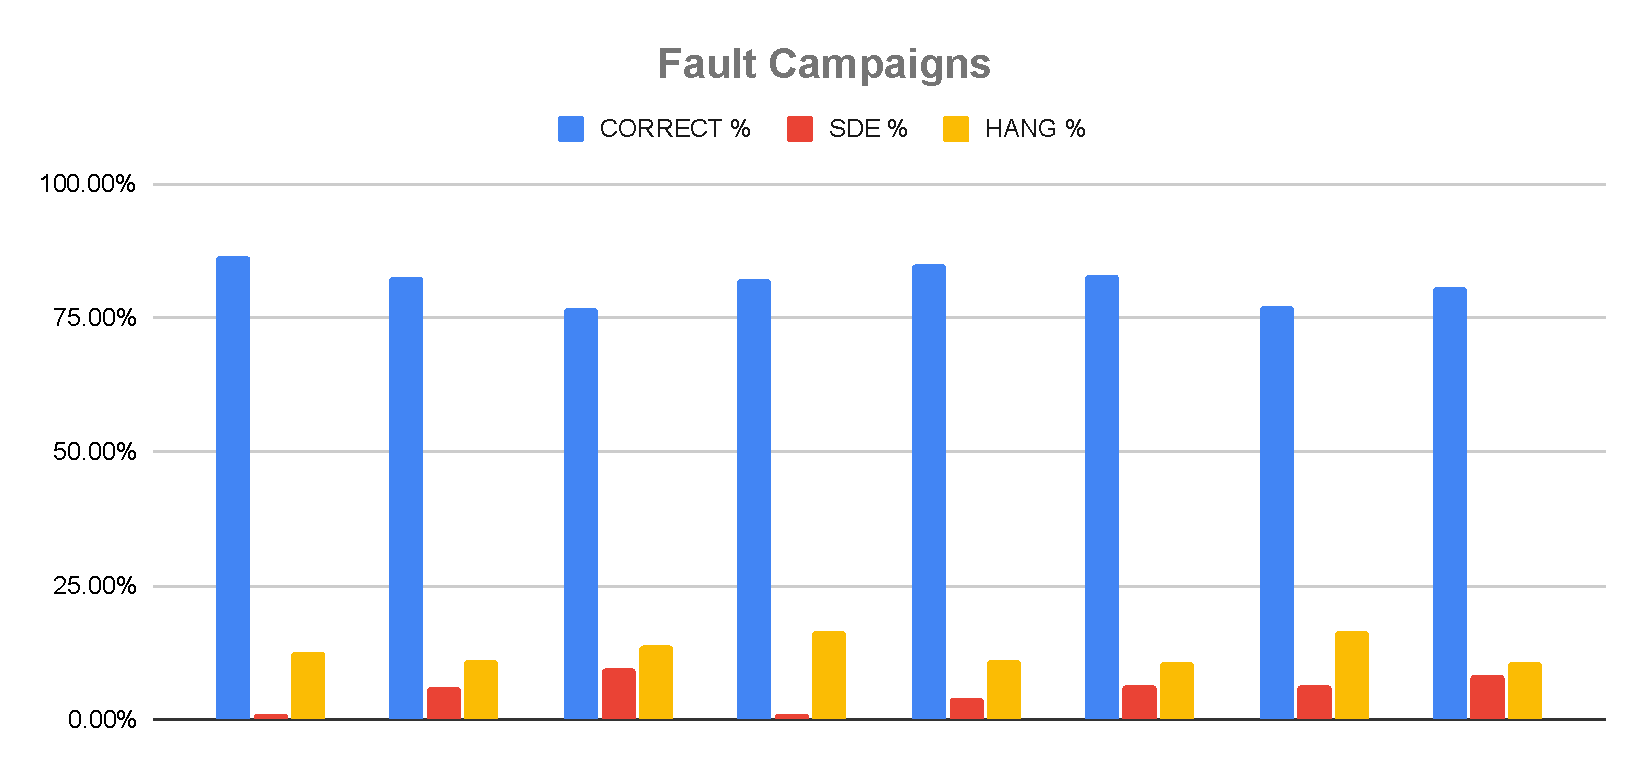
\includegraphics[width=0.95\linewidth]{images/chapter5/chart.pdf}
\caption{Chart representing the executed Fault Injection campaigns.}
\end{figure}

The blue ones are the correct results. The total correct results among all the campaigns is 626, 65 of which have been corrected by the fault tolerance system. Among the red ones representing SDEs, the total is 41. Among these 41 SDEs, 12 have been successfully corrected, while the other 29 have not been corrected.\bigskip

Among these 29 not corrected SDEs, 8 have been detected but the system could not fix them, while the remaining 21 have not been detected at all. This can be easily fixed by increasing the quality of self-test routines in the firmware, looking for example for differences in the produced UART output and the expected one or by comparing written memory values with the expected ones. Consequently, this may help in increasing the coverage of those faults. \bigskip

The remaining yellow cases represents situations where the MicroBlaze is completely halted, even after one or multiple reconfigurations have been performed. There is a total of 99 hangs, 9 of which have not been detected at all. As the not detected SDEs, this can be fixed by increasing the quality of self-test routines. The remaining cases are the uncoverable ones. \bigskip

As a side note, the unrecoverable cases are particular cases where it is not possible to say if the overall fault tolerance system is working or not. Unfortunately, the bitstreams cannot be fully controllable and the fault injection tools randomly injects bit flips in an area that is thought to be 100\% dedicated to the MicroBlaze but it is not true. A bitflip could affect a configuration instruction instead of a configuration bit, leading to a misconfiguration anywhere else in the overall FPGA, thus it cannot be fixed by the partial reconfiguration.

% First of all, it is important to understand how the fault-injection campaigns have been conducted, in order to better comprehend the results and their importance. An important question that I faced while starting these campaigns was: how many injections are enough? To take this decision, several campaigns with increasing number of injections have been conducted and the results were varying until around 10’000 injections. Above this limit, the obtained results were stable around certain values. Trying also with different fault models, the behaviour was pretty much the same, so it has been decided to choose 10’000 as minimum number of injections for each of the campaign.

